%jako, że ma tu być podział chronologiczny, musicie pisać swoje części w osobnych plikach, a ja dokonam podziału chronologicznego i zmerge'uję to samodzielnie. Sądzę, że jest to znacznie bezpieczniejsze rozwiązanie, niż zabawa w merge'owanie jednego pliku u 4 osób w sposób rozproszony...
\subsection{Mapowanie obiektowo-relacyjne}
%label do uzupełnienia po merge'u
Mapowanie obiektowo-relacyjne pozwala uprościć operacje na danych przechowywanych w bazie danych poprzez udostępnienie ich programiście w postaci obiektowej.\\
System \emph{iQuest} operuje na klasach takich jak: ankieta, badanie, grupa docelowa, członek grupy docelowej, uprawnienie dostępu, pytanie (i potomne), odpowiedź, zadanie, praca w tle, etc. Początkowo architekt stworzył diagram klas na którym każda klasa miała wyróżnione publiczne metody \emph{insert, update, delete}. Niestety takie rozwiązanie spowodowało powielenie dużej ilości kodu związanego z interakcją z bazą danych. W ramach refaktoryzacji podjąłem się zadania stworzenia klas, które wzorem nowoczesnych systemów \emph{ORM} uproszczą projektowanie nowych klas reprezentujących dane. Ze względu na silną integrację z mechanizmami \emph{Moodle} w grę nie wchodziły gotowe rozwiązania. Autorskie rozwiązanie korzysta z mechanizmów \emph{Moodle Data manipulation API} oraz mechanizmu refleksji języka PHP, by pozwolić programiście korzystającego z tego rozwiązania na proste pobieranie i manipulację obiektami przechowywanymi w bazie danych. Diagram UML przedstawia się następująco:
\begin{figure}[H]
\begin{center}
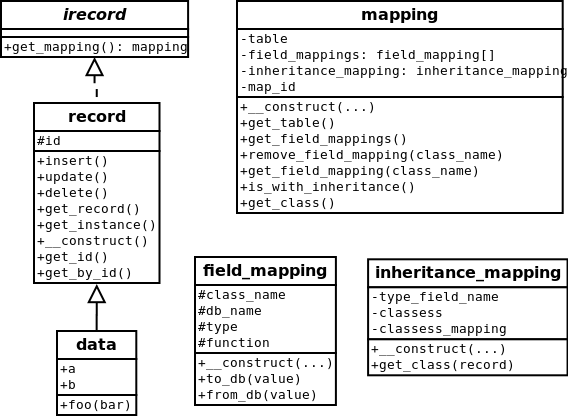
\includegraphics[width=0.9\textwidth]{figures/lw/iquest-orm.png} 
\end{center}
\caption{iQuest ORM}
\label{fig:iquest-orm}
\end{figure}
Klasa danych dziedziczy po klasie \emph{record} oraz implementuje metodę \emph{get\_mapping} interfejsu \emph{irecord}, by uzyskać dostęp do metod komunikacji z bazą danych. Metoda \emph{get\_mapping} pozwala zdefiniować mapowanie danej klasy na odpowiednią relację w bazie danych. Należy przy tym podać mapowania dla atrybutów, tj. nazwy w klasie i bazie danych oraz typ, który zadecyduje o metodzie pobrania/zapisania danej (typem może być także klasa potomna klasy \emph{record}). W przypadku, gdy mamy do czynienia z dziedziczeniem wystarczy zdefiniować przy mapowaniu sposób obsługi dziedziczenia (m.in. jakie pole określa typ klasy). Najważniejszy kod znajduje się w metodzie \emph{get\_instance}, która pobiera konstruktor danej klasy, poprzez refleksję tworzy obiekt z wyłuskanymi z bazy danych parametrami wymaganymi przy jego tworzeniu oraz ustawia resztę pól pobranych z bazy danych. Metody \emph{insert, update, delete} pobierają reprezentację obiektu oczekiwanego przez metody \emph{Data manipulation API} oraz wykonują żądane operacje.\\
Zastosowane rozwiązanie znacząco poprawiło czytelność kodu poprzez zastosowanie zasady DRY (\emph{Don't repeat yourself}). Projektowałem je, mając na uwadze rozwiązanie, z którym miałem wcześniej styczność, tj. implementację \emph{ActiveRecord} z \emph{Ruby on Rails}. W trakcie pracy nad projektem doceniłem stosowanie konwencji nazewniczych, których obecność znacząco upraszcza projektowanie klas mapujących dane.